\documentclass[12pt]{article}
\usepackage[a4paper,left=1.5cm,right=1.5cm,top=1.5cm,bottom=1.5cm]{geometry}
\usepackage[utf8]{inputenc}
\usepackage[T1]{fontenc}	
\usepackage[brazil]{babel}
\usepackage{array,latexsym}
\usepackage{amsmath,amsfonts,amssymb,amsthm,mathabx,amstext}
\usepackage{graphicx}	
\begin{document}
	
	\begin{figure}[h!]
		
\includegraphics[scale=1]{ufpbde}
	\end{figure}
\par \textbf{Nome:} \underline{Paulo Ricardo Seganfredo Campana} \hspace{+12pt} \textbf{Matricula:} \underline{20210044220} \hspace{+12pt} \textbf{Nota:} 

\vspace{+12pt}

	\begin{figure}[h!]
		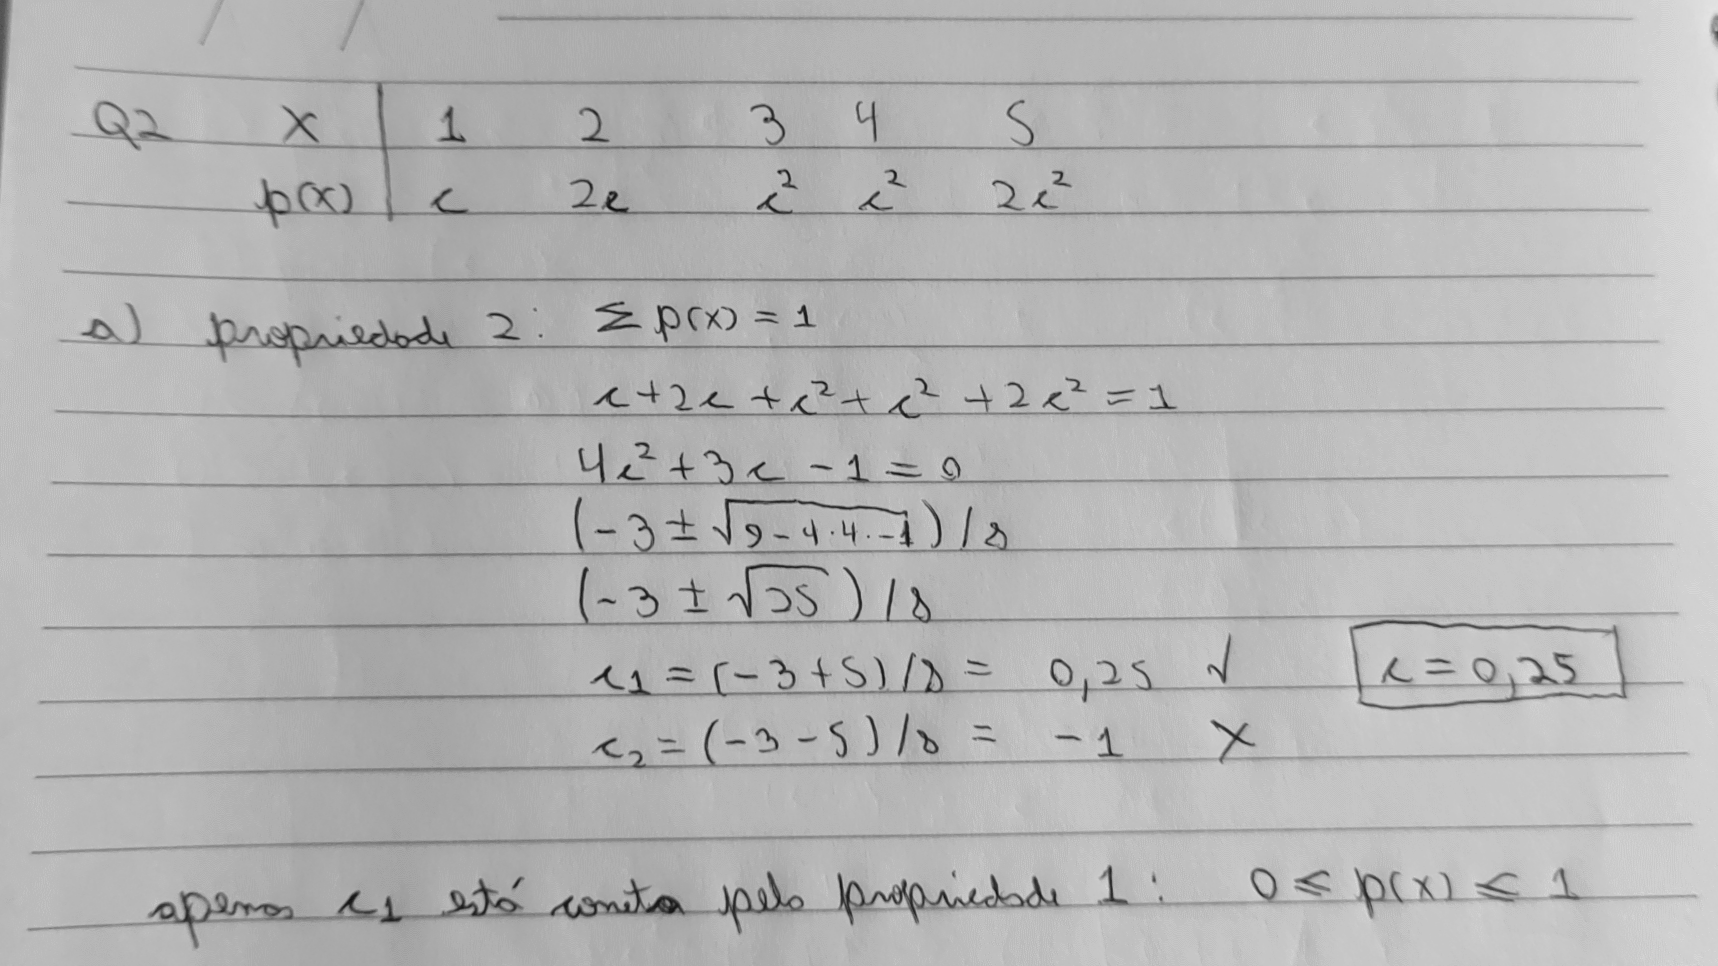
\includegraphics[scale=0.4]{q2a}
	\end{figure}
\vspace{+12pt}

	\begin{figure}[h!]
		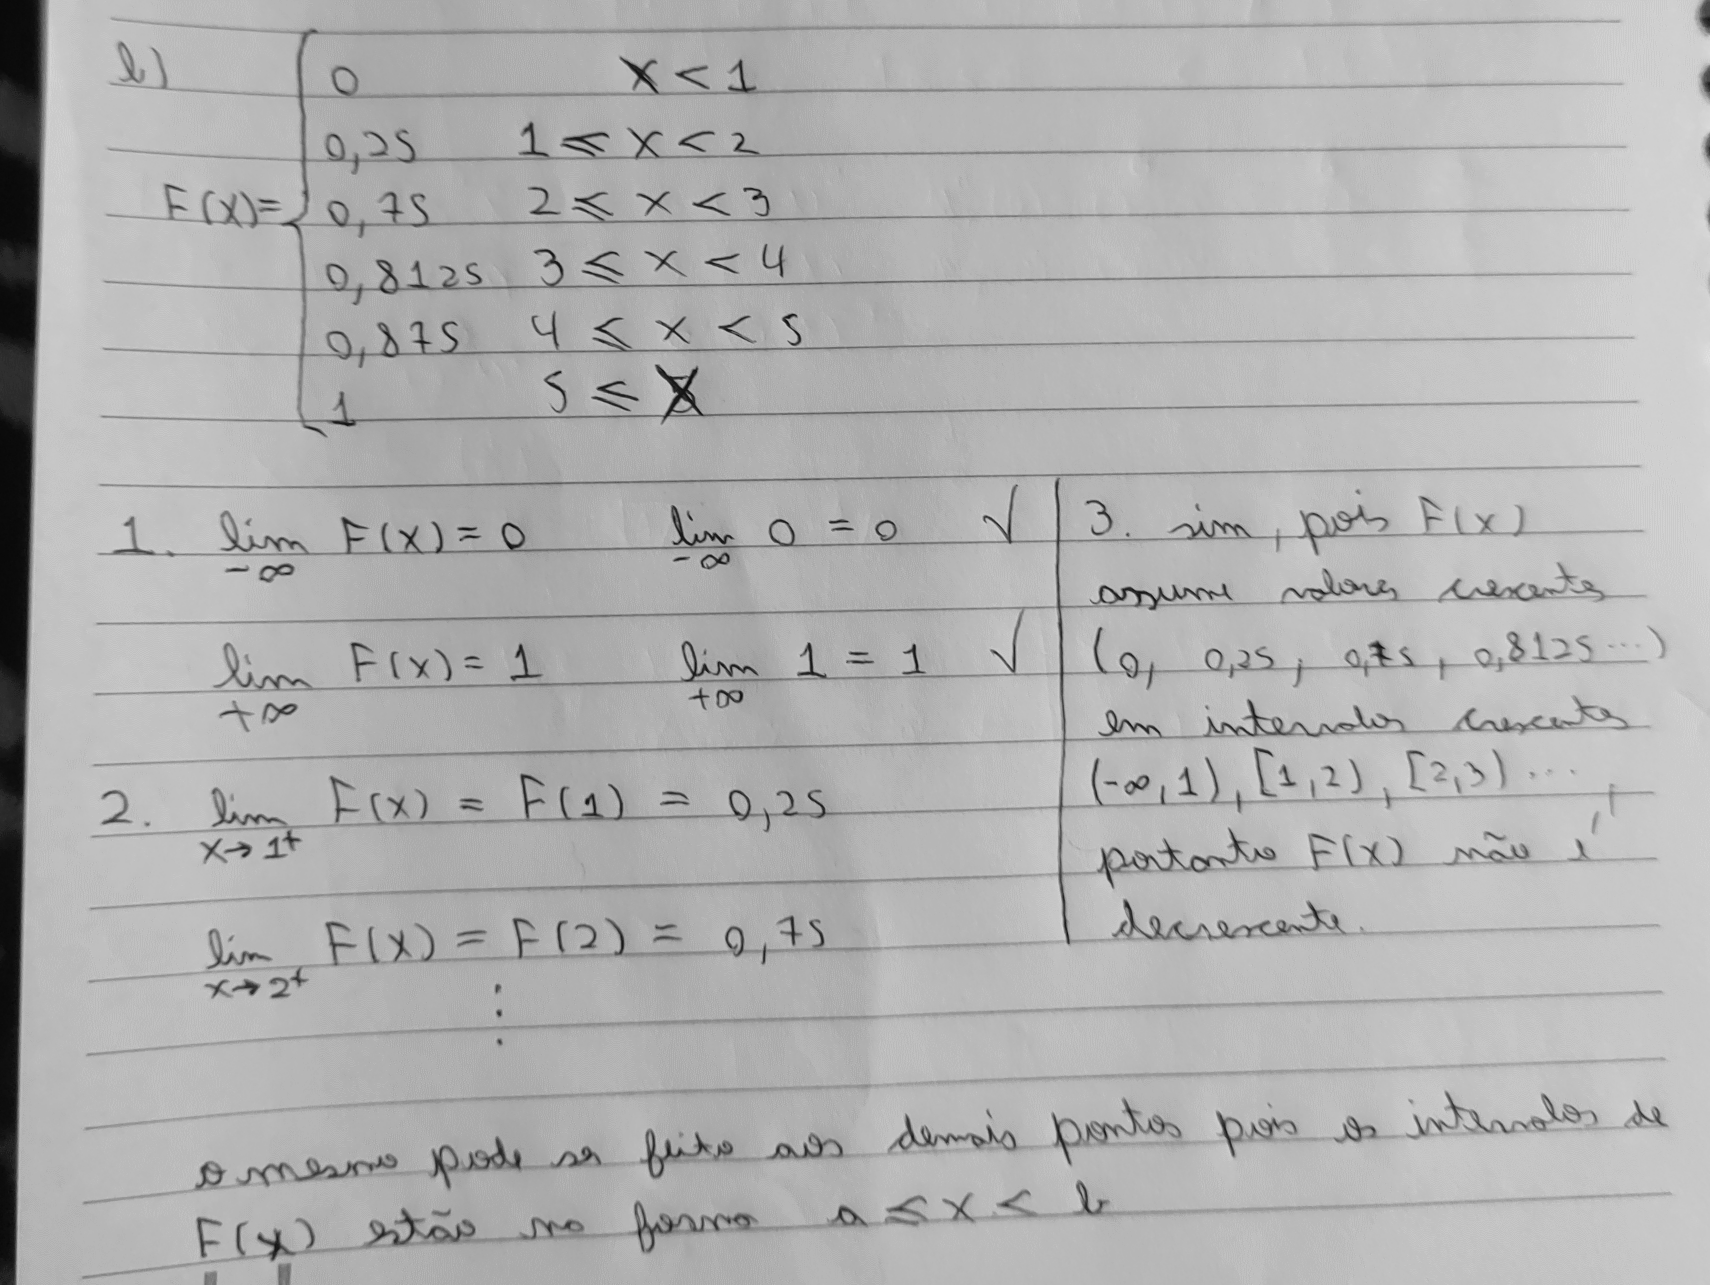
\includegraphics[scale=0.4]{q2b}
	\end{figure}
\vspace{+12pt}

	\begin{figure}[h!]
		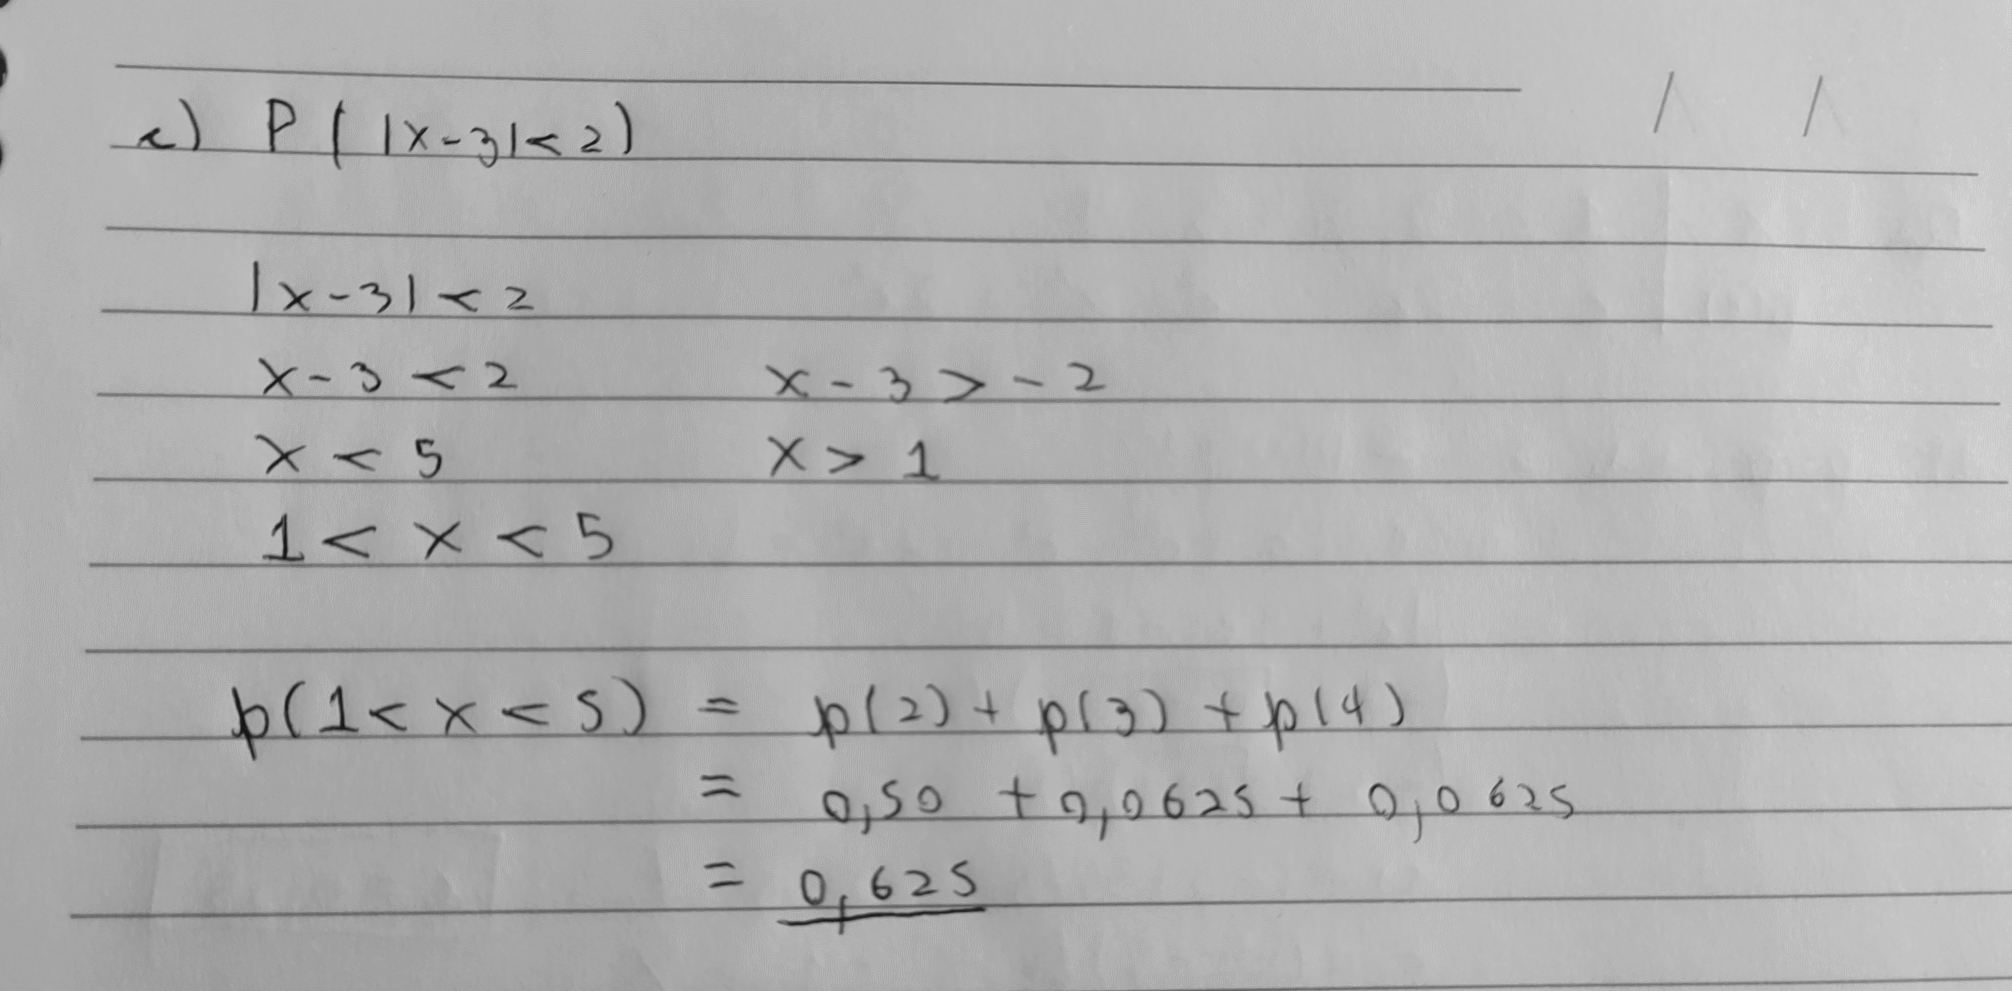
\includegraphics[scale=0.33]{q2c}
	\end{figure}
\vspace{+12pt}

	\begin{figure}[h!]
		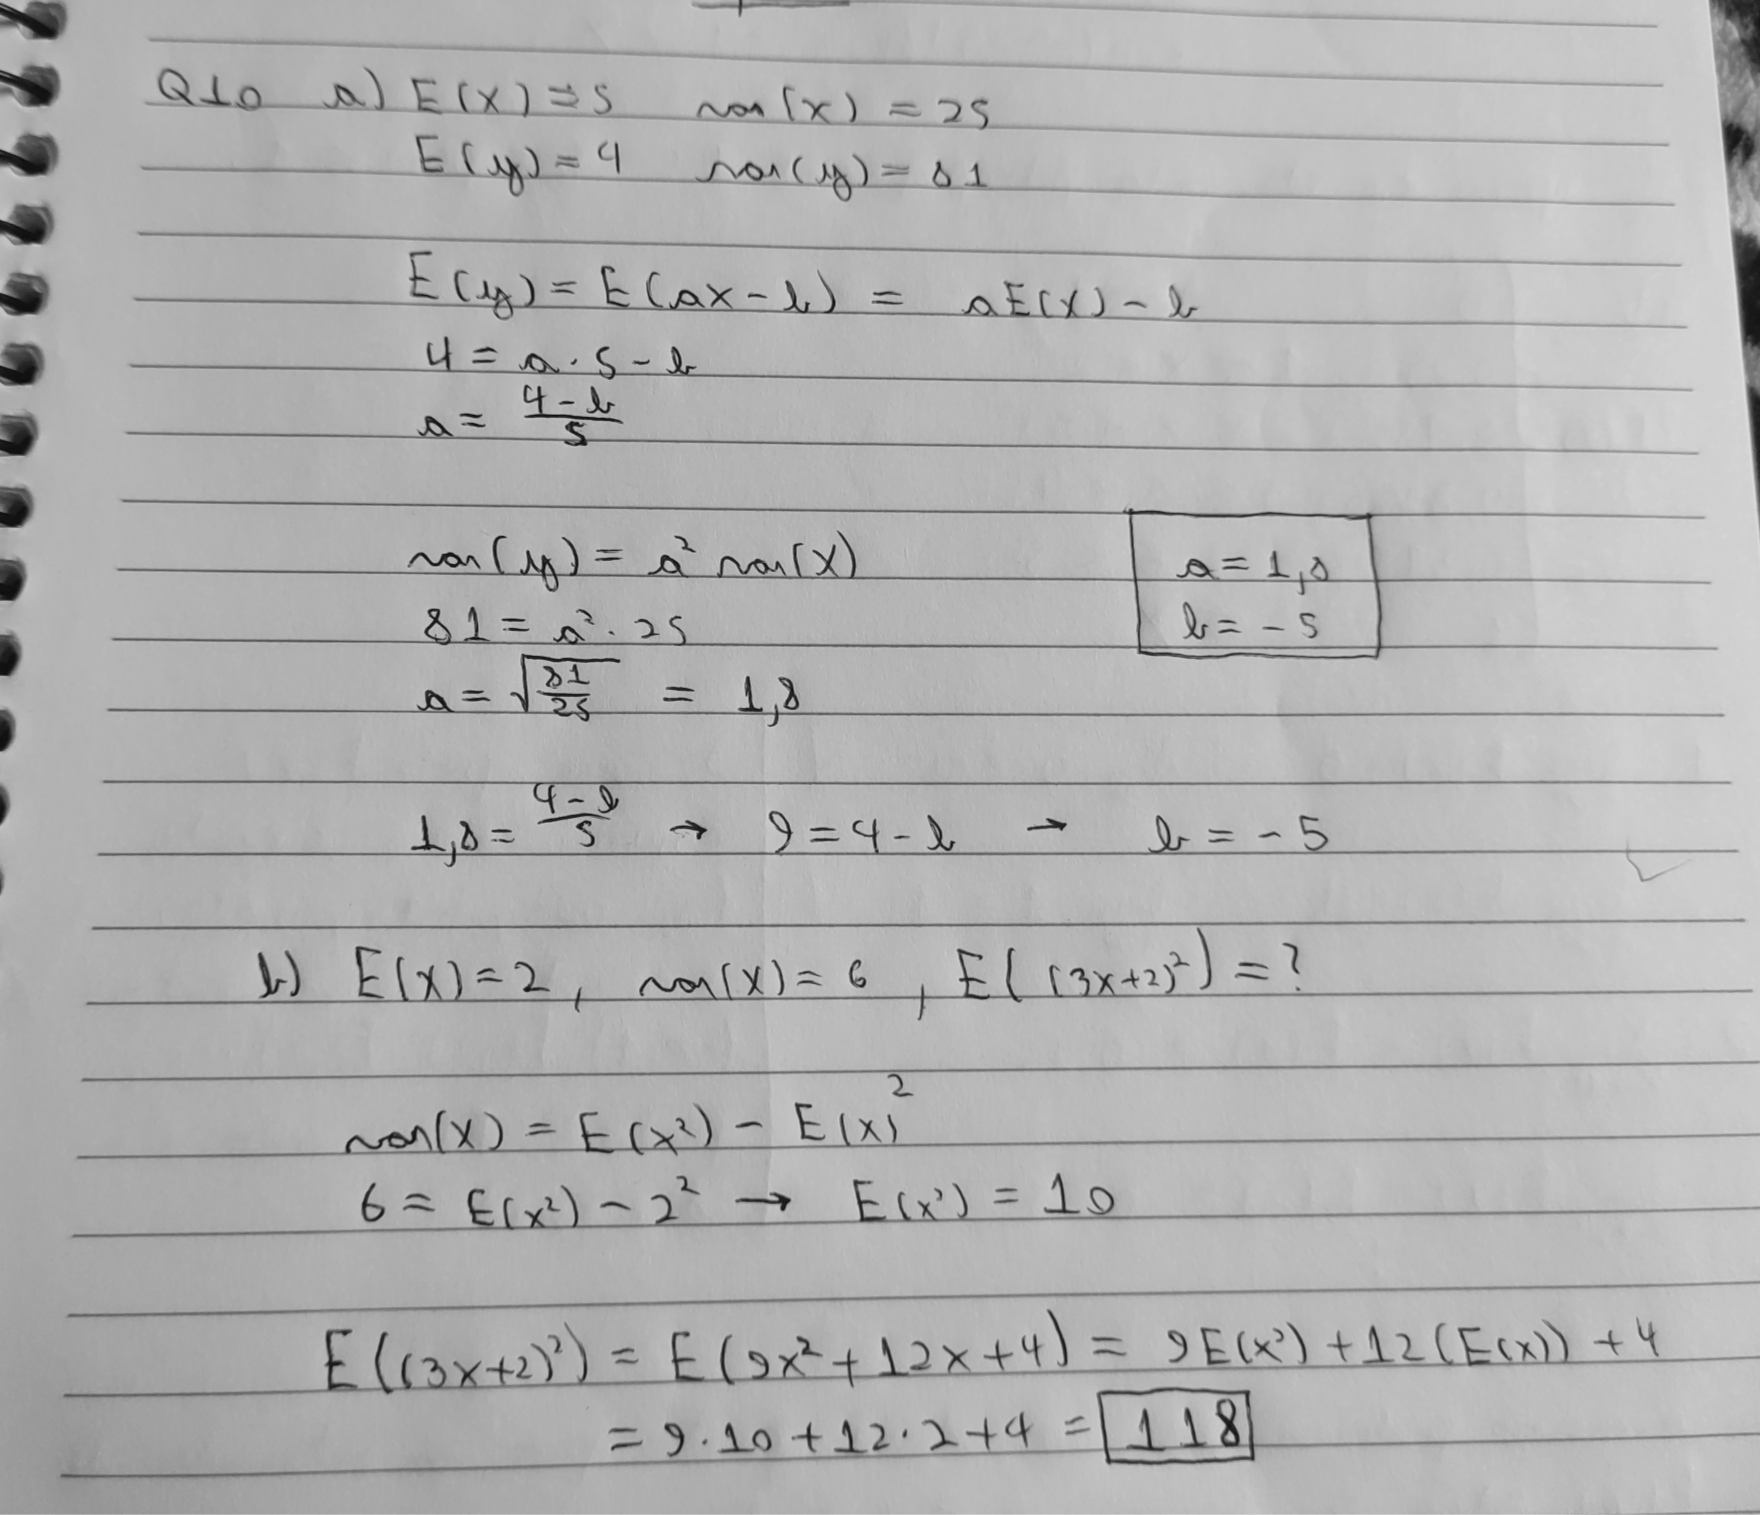
\includegraphics[scale=0.38]{q10}
	\end{figure}
\vspace{+12pt}	

	\begin{figure}[h!]
		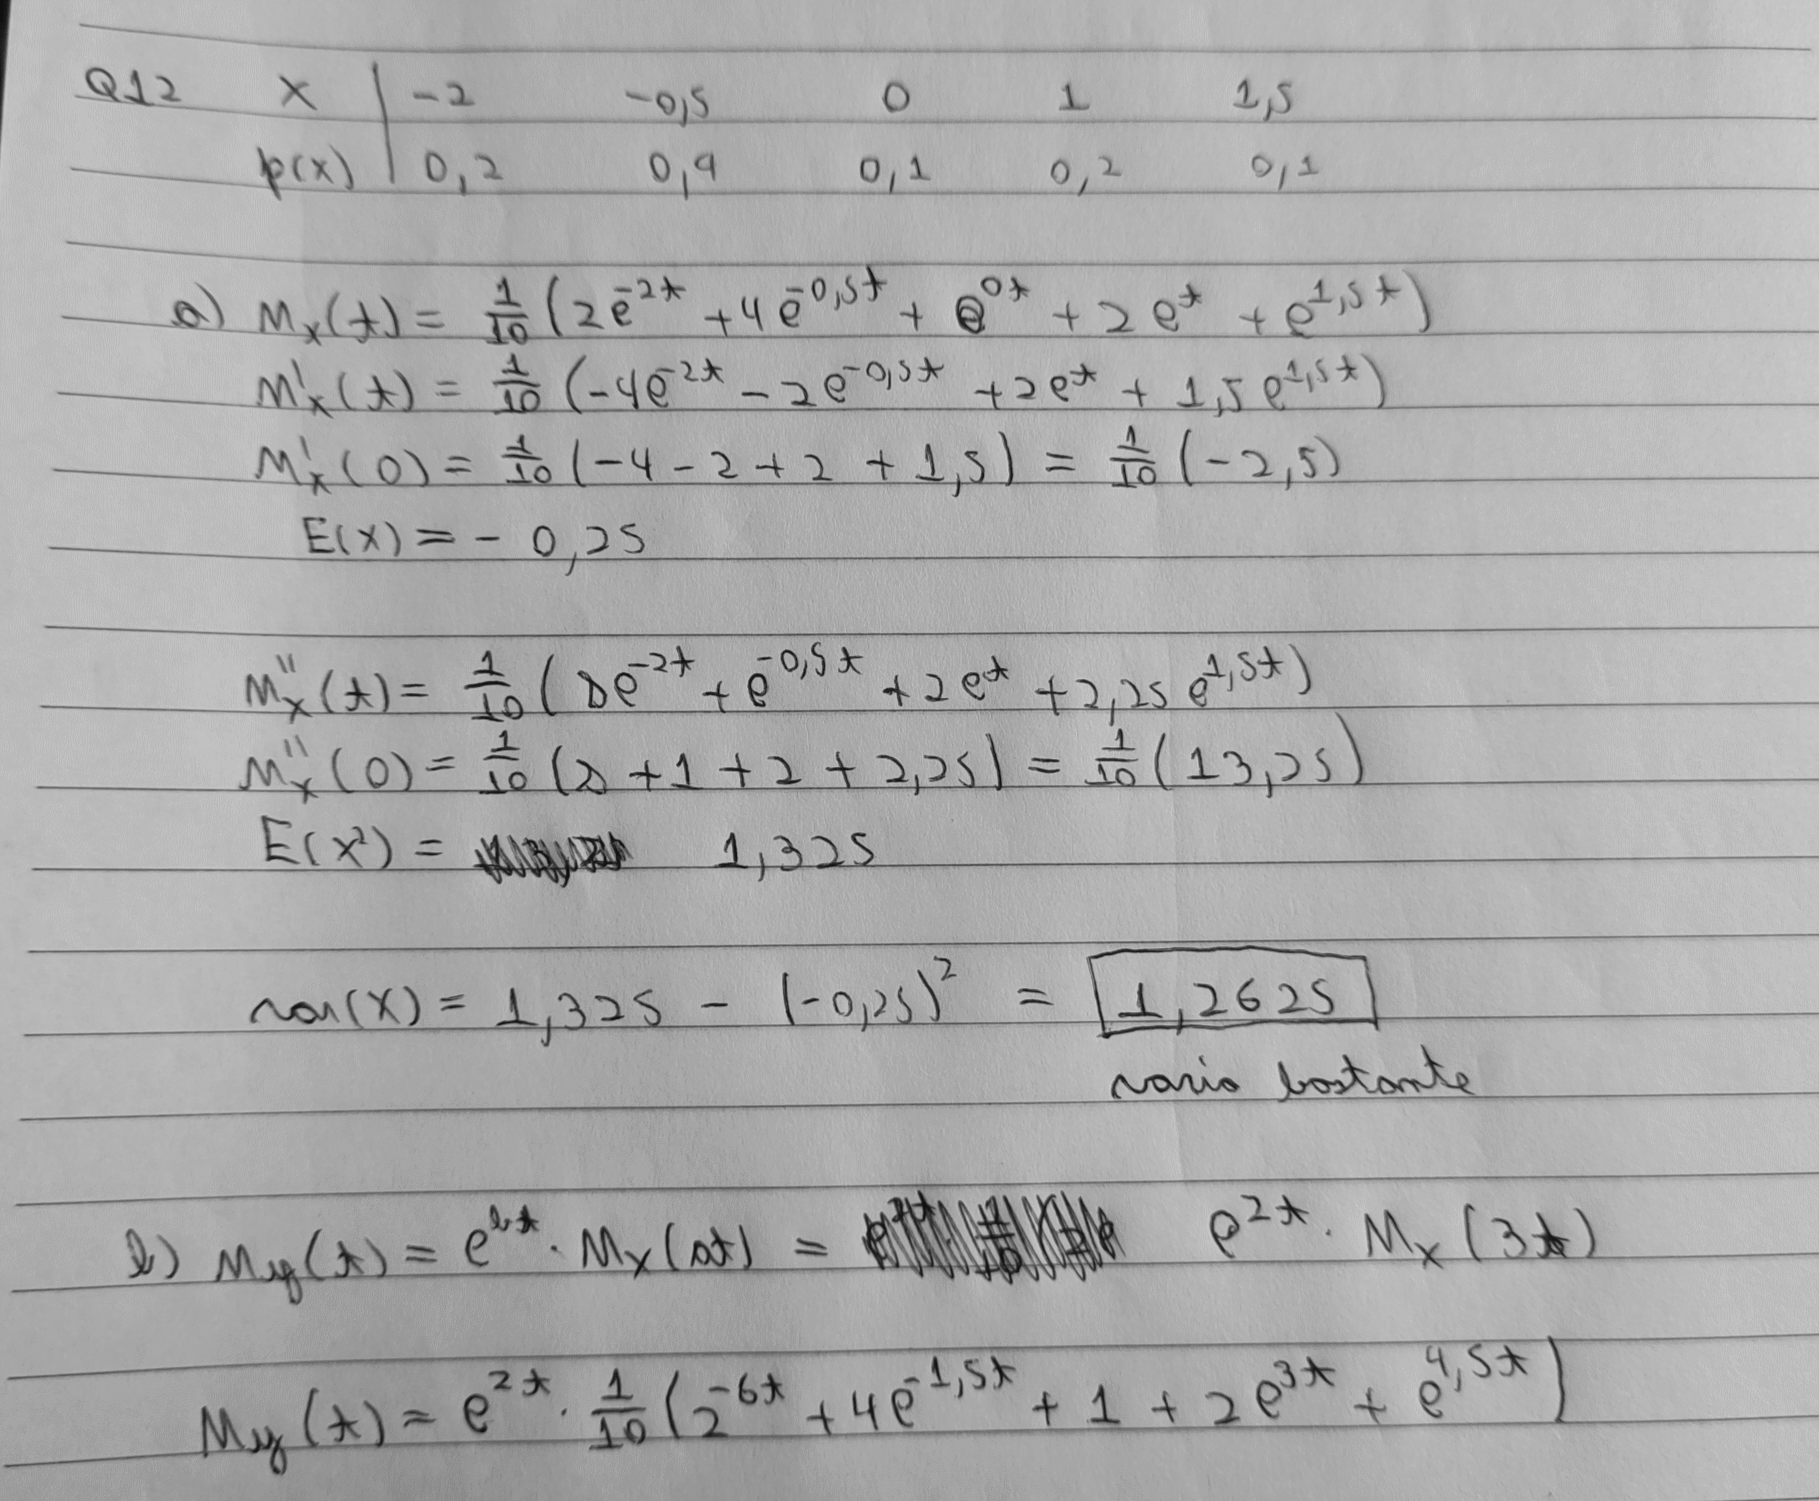
\includegraphics[scale=0.37]{q12}
	\end{figure}
\vspace{+12pt}	

	\begin{figure}[h!]
		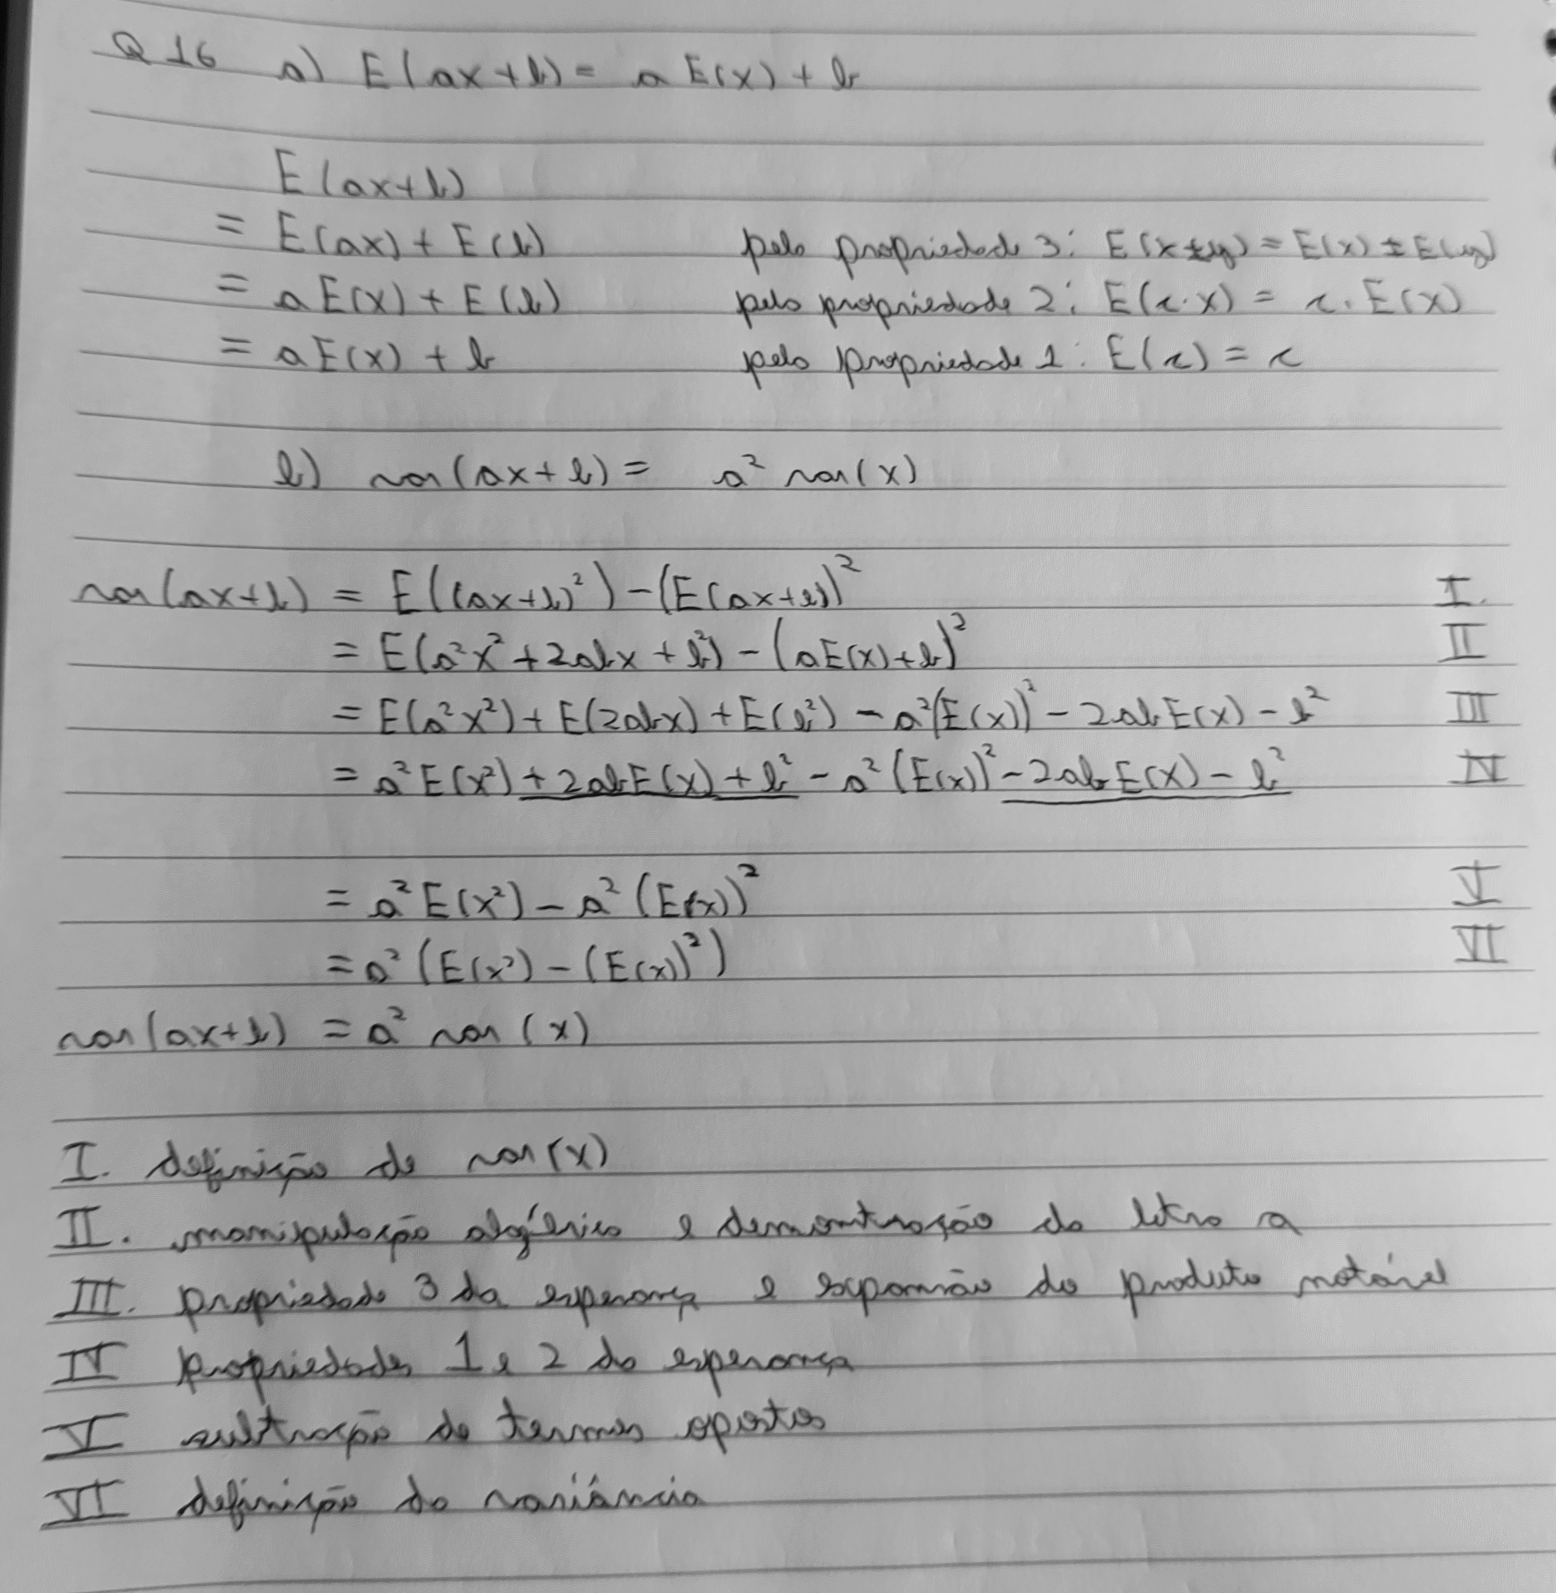
\includegraphics[scale=0.43]{q16}
	\end{figure}

\end{document}